\documentclass[a4paper,10pt]{article}
\usepackage[brazilian]{babel}
\usepackage[left=2.5cm,right=2.5cm,top=3cm,bottom=2.5cm]{geometry}
\usepackage{mathtools}
\usepackage{amsthm}
\usepackage{amsmath}
%\usepackage{nccmath}
\usepackage{amssymb}
\usepackage{amsfonts}
\usepackage{physics}
%\usepackage{dsfont}
%\usepackage{mathrsfs}

\usepackage{titling}
\usepackage{indentfirst}

\usepackage{bm}
\usepackage[dvipsnames]{xcolor}
\usepackage{cancel}

\usepackage{xurl}
\usepackage[colorlinks=true]{hyperref}

\usepackage{float}
\usepackage{graphicx}
%\usepackage{tikz}
\usepackage{caption}
\usepackage{subcaption}

%%%%%%%%%%%%%%%%%%%%%%%%%%%%%%%%%%%%%%%%%%%%%%%%%%%

\newcommand{\eps}{\epsilon}
\newcommand{\vphi}{\varphi}
\newcommand{\cte}{\text{cte}}

\newcommand{\N}{\mathbb{N}}
\newcommand{\Z}{\mathbb{Z}}
\newcommand{\Q}{\mathbb{Q}}
\newcommand{\R}{\vb{R}}
\newcommand{\C}{\mathbb{C}}
\renewcommand{\S}{\hat{S}}
%\renewcommand{\H}{\s{H}}

\renewcommand{\a}{\vb{a}}
\newcommand{\nn}{\hat{n}}
\renewcommand{\d}{\dagger}
\newcommand{\up}{\uparrow}
\newcommand{\down}{\downarrow}

\newcommand{\0}{\vb{0}}
%\newcommand{\1}{\mathds{1}}
\newcommand{\E}{\vb{E}}
\newcommand{\B}{\vb{B}}
\renewcommand{\v}{\vb{v}}
\renewcommand{\r}{\vb{r}}
\renewcommand{\k}{\vb{k}}
\newcommand{\p}{\vb{p}}
\newcommand{\q}{\vb{q}}
\newcommand{\F}{\vb{F}}

\newcommand{\s}{\sigma}
%\newcommand{\prodint}[2]{\left\langle #1 , #2 \right\rangle}
\newcommand{\cc}[1]{\overline{#1}}
\newcommand{\Eval}[3]{\eval{\left( #1 \right)}_{#2}^{#3}}

\newcommand{\unit}[1]{\; \mathrm{#1}}

\newcommand{\n}{\medskip}
\newcommand{\e}{\quad \mathrm{e} \quad}
\newcommand{\ou}{\quad \mathrm{ou} \quad}
\newcommand{\virg}{\, , \;}
\newcommand{\ptodo}{\forall \,}
\renewcommand{\implies}{\; \Rightarrow \;}
%\newcommand{\eqname}[1]{\tag*{#1}} % Tag equation with name

\setlength{\droptitle}{-7em}

\theoremstyle{plain}
\newtheorem{theorem}{Teorema}[section]
%\newtheorem{defi}[theorem]{Definição}
\newtheorem{lemma}[theorem]{Lema}
%\newtheorem{corol}[theorem]{Corolário}
%\newtheorem{prop}[theorem]{Proposição}
%\newtheorem{example}{Exemplo}
%
%\newtheorem{inneraxiom}{Axioma}
%\newenvironment{axioma}[1]
%  {\renewcommand\theinneraxiom{#1}\inneraxiom}
%  {\endinneraxiom}
%
%\newtheorem{innerpostulado}{Postulado}
%\newenvironment{postulado}[1]
%  {\renewcommand\theinnerpostulado{#1}\innerpostulado}
%  {\endinnerpostulado}
%
%\newtheorem{innerexercise}{Exercício}
%\newenvironment{exercise}[1]
%  {\renewcommand\theinnerexercise{#1}\innerexercise}
%  {\endinnerexercise}
%
%\newtheorem{innerthm}{Teorema}
%\newenvironment{teorema}[1]
%  {\renewcommand\theinnerthm{#1}\innerthm}
%  {\endinnerthm}
%
\newtheorem{innerlema}{Lema}
\newenvironment{lema}[1]
  {\renewcommand\theinnerlema{#1}\innerlema}
  {\endinnerlema}
%
%\theoremstyle{remark}
%\newtheorem*{hint}{Dica}
%\newtheorem*{notation}{Notação}
%\newtheorem*{obs}{Observação}


\setlength\parindent{0pt}  % noindent in entire file

\usepackage{minted}
\usemintedstyle{vs}
\definecolor{bg}{rgb}{0.85,0.85,0.85}
\setmintedinline{bgcolor=bg}
\newcommand{\python}[1]{\mintinline{python}{#1}}
\usepackage{tcolorbox}
\tcbuselibrary{minted,skins}
\newtcblisting{Python}{
  listing engine=minted,
  colback=bg,
  colframe=black!70,
  listing only,
  minted style=vs,
  minted language=python,
  minted options={texcl=true, fontsize=\scriptsize},
  left=1mm,
}

\renewcommand{\p}{\phantom{+}}
\newcommand{\mchi}{\chi^{\Gamma^\pi_{p_z}}}
\renewcommand{\c}[1]{\textcolor{red}{#1}}

\title{\Huge{\textbf{Teoria de grupos - Exercício 4}}}
\author{Mateus Marques}

\begin{document}

\maketitle

\section*{A ligação $\pi$ e a fatoração da equação secular da molécula de naftaleno C$_{10}$H$_8$}

Primeiramente determinaremos o grupo de simetria da molécula de naftaleno, esboçado na Figura \ref{fig:D2h}:
$$
\text{não é linear} \implies \text{eixo }C_{2z} \implies \text{não tem }S_{4} \implies
\text{2 eixos }C_2 \perp C_{2z} \implies \sigma_h \implies \boxed{\text{grupo }D_{2h}.}
$$
\begin{figure}[H]
\centering
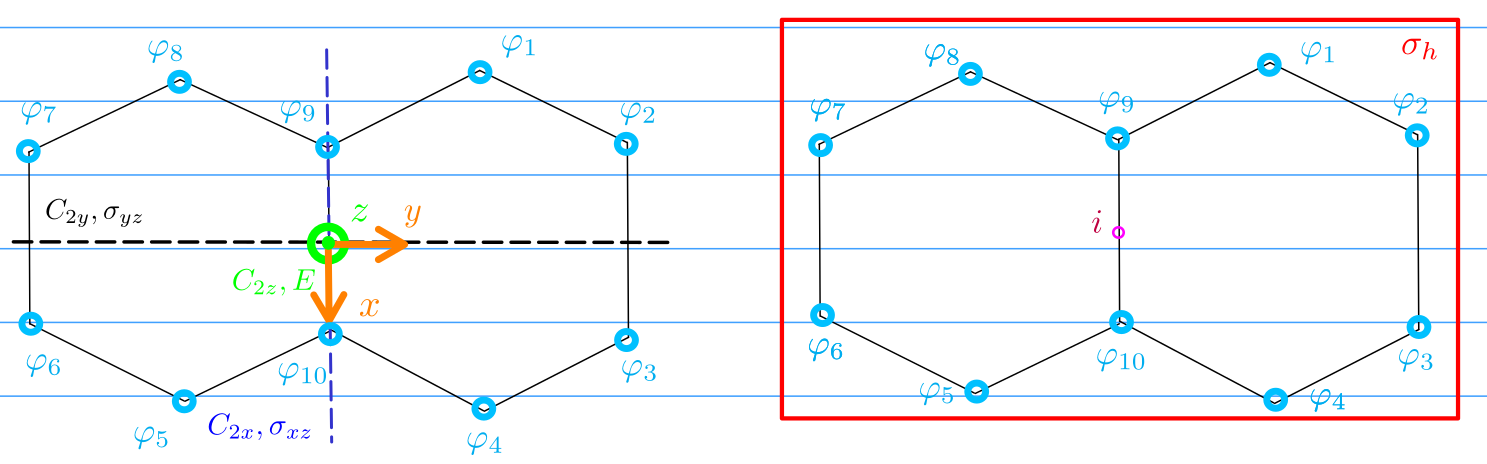
\includegraphics[width=1.0\linewidth]{fig/D2h.png}
\caption{Elementos de simetria do grupo $D_{2h}$, correspondente à molécula de naftaleno C$_{10}$H$_8$.}
\label{fig:D2h}
\end{figure}

O grupo é $D_{2h} = \{E, C_{2z}, C_{2y}, C_{2x}, i, \sigma_h, \sigma_{xz}, \sigma_{yz}\}$, e os elementos estão desenhados na Figura \ref{fig:D2h}.

\n

Agora descobriremos a representação $\Gamma^\pi_{p_z}$. Note que a base tem dimensão $10$, já que temos 10 orbitais, representados pelo vetor $(\vphi_1, \vphi_2, \vphi_3, \vphi_4, \vphi_5, \vphi_6, \vphi_7, \vphi_8, \vphi_9, \vphi_{10})$. Avaliaremos os caracteres dessa representação $\Gamma^\pi_{p_z}$ para seus elementos, seguindo os desenhos da Figura \ref{fig:D2h}:
\begin{enumerate}
\item $E$ $\implies$ mantém os 10 orbitais, portanto $\mchi(E) = 10$.
\item $C_{2z}$ $\implies$ troca os 10 orbitais de lugar, portanto $\mchi(C_{2z}) = 0$.
\item $C_{2y}$ $\implies$ troca os 10 orbitais de lugar, portanto $\mchi(C_{2y}) = 0$.
\item $C_{2x}$ $\implies$ troca 8 orbitais de lugar e inverte a polarização de 2, portanto $\mchi(C_{2x}) = -2$.
\item $i$ $\implies$ troca os 10 orbitais de lugar, portanto $\mchi(i) = 0$.
\item $\sigma_{h}$ $\implies$ inverte a polarização dos 10 orbitais, portanto $\mchi(\sigma_{h}) = -10$.
\item $\sigma_{xz}$ $\implies$ troca 8 orbitais de lugar e mantém os 2 restantes, portanto $\mchi(\sigma_{xz}) = 2$.
\item $\sigma_{yz}$ $\implies$ troca os 10 orbitais de lugar, portanto $\mchi(\sigma_{yz}) = 0$.
\end{enumerate}

Retirando a tabela de caracteres do grupo $D_{2h}$ do site \url{http://symmetry.jacobs-university.de/cgi-bin/group.cgi?group=602&option=4} e adicionando a linha com os caracteres de $\Gamma^\pi_{p_z}$, obtemos a Tabela \ref{tab:mult_D2h} abaixo.

\begin{table}[H]
\caption{Tabela de caracteres para o grupo $D_{2h}$.}
\centering

\begin{tabular} { |c|c c c c c c c c | }
\hline
$D_{2h}$ & $E$ & $C_{2z}$ & $C_{2y}$ & $C_{2x}$ & $i$ & $\sigma_{h}$ & $\sigma_{xz}$ & $\sigma_{yz}$ \\
\hline
$A_{g}$                      & $\p1$ & $\p1$ & $\p1$ & $\p1$ & $\p1$ & $\p1$ & $\p1$ & $\p1$ \\
$B_{1g}$                     & $\p1$ & $\p1$ & $ -1$ & $ -1$ & $\p1$ & $\p1$ & $ -1$ & $ -1$ \\
$\c{\boxed{3\times B_{2g}}}$ & $\c{\p1}$ & $\c{ -1}$ & $\c{\p1}$ & $\c{ -1}$ & $\c{\p1}$ & $\c{ -1}$ & $\c{\p1}$ & $\c{ -1}$ \\
$\c{\boxed{2\times B_{3g}}}$ & $\c{\p1}$ & $\c{ -1}$ & $\c{ -1}$ & $\c{\p1}$ & $\c{\p1}$ & $\c{ -1}$ & $\c{ -1}$ & $\c{\p1}$ \\
$\c{\boxed{2\times A_{u}}}$  & $\c{\p1}$ & $\c{\p1}$ & $\c{\p1}$ & $\c{\p1}$ & $\c{ -1}$ & $\c{ -1}$ & $\c{ -1}$ & $\c{ -1}$ \\
$\c{\boxed{3\times B_{1u}}}$ & $\c{\p1}$ & $\c{\p1}$ & $\c{ -1}$ & $\c{ -1}$ & $\c{ -1}$ & $\c{ -1}$ & $\c{\p1}$ & $\c{\p1}$ \\
$B_{2u}$                     & $\p1$ & $ -1$ & $\p1$ & $ -1$ & $ -1$ & $\p1$ & $ -1$ & $\p1$ \\
$B_{3u}$                     & $\p1$ & $ -1$ & $ -1$ & $\p1$ & $ -1$ & $\p1$ & $\p1$ & $ -1$ \\
\hline
\hline
$\Gamma_{p_z}^\pi$ & $\p10$ & $\p0$ & $\p0$ & $ -2$ & $\p0$ & $-10$ & $\p2$ & $\p0$ \\
\hline
\end{tabular}

\label{tab:mult_D2h}
\end{table}

Analisando a Tabela \ref{fig:D2h} com cuidado, vemos que a representação redutível $\Gamma^\pi_{p_z}$ se decompõe exatamente da forma
$$
\boxed{ \Gamma^\pi_{p_z} = 3 B_{2g} \oplus 2 B_{3g} \oplus 2 A_{2u} \oplus 3 B_{1u}. }
$$

Agora basta aplicarmos os operadores de projeção para obter os orbitais simetrizados. Sendo $\Gamma$ uma das representações irredutíveis, o operador de projeção $\mathcal{P}^{(\Gamma)}$ é dado por
\begin{equation} \label{eq:projection}
\mathcal{P}^{(\Gamma)} = \frac{\ell_{\Gamma}}{h} \sum_{R \in G} \chi^{(\Gamma)}(R) P_R,
\end{equation}
onde $\ell_\Gamma$ é a dimensão da representação $\Gamma$, $h = 10$ é a ordem do grupo $G = D_{2h}$ e $P_R$ é o operador do elemento de simetria $R \in G$. Queremos utilizar a equação \ref{eq:projection} para calcular $\mathcal{P}^{(\Gamma)} \vphi_i$, para $\Gamma = B_{2g}, B_{3g}, A_{2u}, B_{1u}$. Para isso, precisaremos da ação $P_R \vphi_i$ para cada um dos 8 operadores $R \in D_{2h}$.

As representações irredutíveis em questão são todas unidimensionais, mas são bidegeneradas ($2 B_{3g}$ e $2 A_{2u}$) ou tridegeneradas ($3 B_{2g}$ e $3 B_{1u}$). Portanto, basta que calculemos por exemplo $P_R \vphi_1$, $P_R \vphi_2$, $P_R \vphi_9$ para todo $R \in G$. Assim, montamos a Tabela \ref{tab:proj} com o auxílio da Figura \ref{fig:orbitais_pz-naft} que define os orbitais $p_z$.
\begin{figure}[H]
\centering
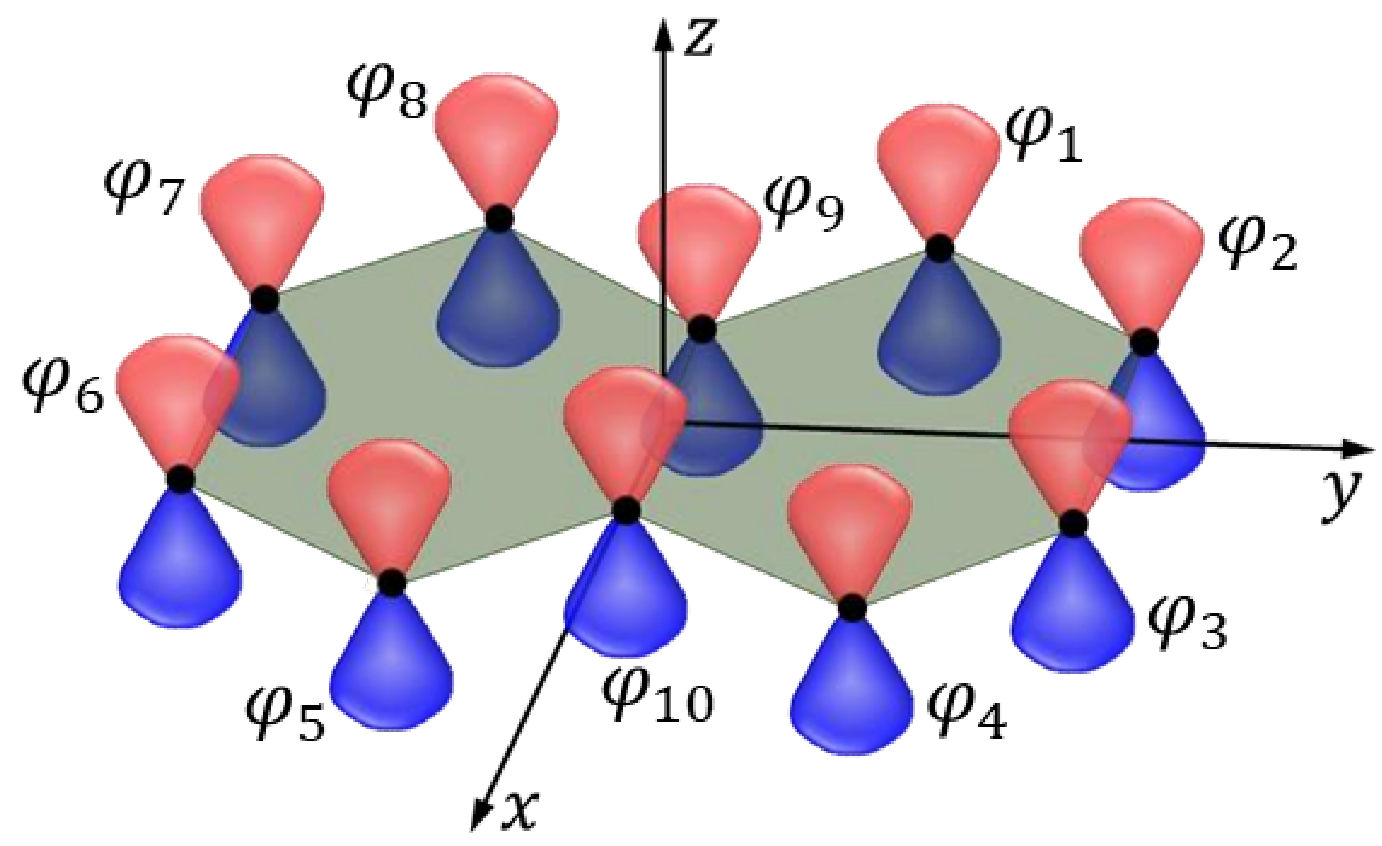
\includegraphics[width=0.6\linewidth]{fig/orbitais_pz-naft.png}
\caption{Orbitais $p_z$ perpendiculares ao plano da molécula de naftaleno C$_{10}$H$_8$.}
\label{fig:orbitais_pz-naft}
\end{figure}


\begin{table}[H]
\caption{Tabela da ação dos operadores $P_R$ nos orbitais $\vphi_1, \vphi_2, \vphi_9$.}
\centering
\footnotesize

\begin{tabular} { | c c | }
\hline
$P_{E} \vphi_1 =  \vphi_1, P_{E} \vphi_2 =   \vphi_2, P_E \vphi_9 = \vphi_9$ & $P_{C_{2z}} \vphi_1 = \vphi_5, P_{C_{2z}} \vphi_2 = \vphi_6, P_{C_{2z}} \vphi_9 = \vphi_{10}$ \\
$P_{C_{2y}} \vphi_1 = -\vphi_4, P_{C_{2y}} \vphi_2 = -\vphi_3, P_{C_{2y}} \vphi_9 = -\vphi_{10}$ & $P_{C_{2x}} \vphi_1 = -\vphi_8, P_{C_{2x}} \vphi_2 = -\vphi_7, P_{C_{2x}} \vphi_9 = -\vphi_9$ \\
$P_{i} \vphi_1 = -\vphi_5, P_{i} \vphi_2 = -\vphi_6, P_{i} \vphi_9 = -\vphi_{10}$ & $P_{\sigma_h} \vphi_1 = -\vphi_1, P_{\sigma_h} \vphi_2 = -\vphi_2, P_{\sigma_h} \vphi_9 = -\vphi_9$ \\
$P_{\sigma_{xz}} \vphi_1 = \vphi_8, P_{\sigma_{xz}} \vphi_2 = \vphi_7, P_{\sigma_{xz}} \vphi_9 = \vphi_9$ & $P_{\sigma_{yz}} \vphi_1 = \vphi_4, P_{\sigma_{yz}} \vphi_2 = \vphi_3, P_{\sigma_{yz}} \vphi_9 = \vphi_{10}$ \\
\hline
\end{tabular}

\label{tab:proj}
\end{table}

Com a Tabela \ref{tab:proj} podemos realizar a soma da equação \ref{eq:projection}. Porém, além disso resultar em muitos cálculos, ainda teremos que ortonormalizar os orbitais. Por isso, preferi reaproveitar o programa em \python{python} que escrevi para resolver o Exercício 3 da molécula de benzeno. Utilizei a biblioteca \python{sympy} para realizar os cálculos simbólicos.

\n

O código utilizado foi:

\begin{Python}
from sympy import symbols, Poly, sqrt, latex
from sympy.matrices import Matrix, GramSchmidt

f1, f2, f3, f4, f5, f6 = symbols('varphi_1 varphi_2 varphi_3 varphi_4 varphi_5 varphi_6')

h = 24  # order of the group
dim = [1, 2, 1, 2]  # the dimensions of the irreps $B_{2g}$, $E_{1g}$, $A_{2u}$, $E_{2u}$

# chi is the 4x24 matrix for the characters from the irreps [$B_{2g}$, $E_{1g}$, $A_{2u}$, $E_{2u}$] and group $D_{6h}$
#         $E$  $2 C_6$    $2 C_3$  $C_2$     $3 C_2'$      $3 C_2''$      $i$    $2 S_3$     $2 S_6$  $\sigma_h$    $3 \sigma_d$     $3 \sigma_v$
chi = [ [ 1, -1,-1,  1, 1, -1,  -1,-1,-1,  1, 1, 1,   1,  -1,-1,   1, 1, -1, -1,-1,-1, 1,1,1, ],     #  $B_{2g}$, index 0
        [ 2,  1, 1, -1,-1, -2,   0, 0, 0,  0, 0, 0,   2,   1, 1,  -1,-1, -2,  0, 0, 0, 0,0,0, ],     #  $E_{1g}$, index 1
        [ 1,  1, 1,  1, 1,  1,  -1,-1,-1, -1,-1,-1,  -1,  -1,-1,  -1,-1, -1,  1, 1, 1, 1,1,1, ],     #  $A_{2u}$, index 2
        [ 2, -1,-1, -1,-1,  2,   0, 0, 0,  0, 0, 0,  -2,   1, 1,   1, 1, -2,  0, 0, 0, 0,0,0, ], ]   #  $E_{2u}$, index 3

class Proj:     # element of symmetry from D\_6h
    def __init__(self, Pf1, Pf2):
        self.P = [Pf1, Pf2]     # action on orbitals $\varphi_1$ and $\varphi_2$

# D6h is a list with 24 elements
#              E               C6             C6\^5            C3            C3\^2             C2
D6h = [ Proj( f1,  f2), Proj( f6,  f1), Proj( f2,  f3), Proj( f5,  f6), Proj( f3,  f4), Proj( f4,  f5),
#            C2'(1)          C2'(2)         C2'(3)         C2''(1)        C2''(2)          C2''(3)
        Proj(-f3, -f6), Proj(-f5, -f2), Proj(-f1, -f4), Proj(-f2, -f1), Proj(-f4, -f3), Proj(-f6, -f5),
#              i              S3             S3\^2             S6           S6\^5            sigma\_h
        Proj(-f4, -f5), Proj(-f5, -f6), Proj(-f3, -f4), Proj(-f6, -f1), Proj(-f2, -f3), Proj(-f1, -f2),
#           sigma\_d(1)     sigma\_d(2)      sigma\_d(3)     sigma\_v(1)      sigma\_v(2)     sigma\_v(3)
        Proj( f2,  f1), Proj( f4,  f3), Proj( f6,  f5), Proj( f1,  f2), Proj( f3,  f4), Proj( f5,  f6),  ]

# irrep is the index 0, 1, 2, 3 for $B_{2g}$, $E_{1g}$, $A_{2u}$, $E_{2u}$
# phi is the index 0, 1 for $\varphi_1$ or $\varphi_2$
def proj_irrep(irrep, phi):
    soma = 0
    for R in range(len(D6h)):
        soma += chi[irrep][R] * D6h[R].P[phi]   # soma da equação (1)
    return soma * dim[irrep] / h

def norm(u):  # norma de um vetor
    soma = 0
    for e in u:
        soma += e**2
    return sqrt(soma)

def normalize(L):   # normaliza um vetor, especificado pela lista L
    norma = norm(L)
    for i in range(len(L)):
        L[i] /= norma

def myappend(psis, proj):   # macro para montar a lista de vetores
    psi = Poly(proj).coeffs()
    normalize(psi)
    psis.append(Matrix(psi))

def get_var(coeffs, vars):  # colocar em formato de variável simbólica do sympy
    var = 0
    for i in range(len(coeffs)):
        var += coeffs[i] * vars[i]
    return var
\end{Python}

\begin{Python}
def main():
    vars = [f1, f2, f3, f4, f5, f6]
    psis = []
    myappend(psis, proj_irrep(0, 0))    # $\mathcal{P}^{(B_{2g})} \varphi_1$
    myappend(psis, proj_irrep(1, 0))    # $\mathcal{P}^{(E_{1g})} \varphi_1$
    myappend(psis, proj_irrep(1, 1))    # $\mathcal{P}^{(E_{1g})} \varphi_2$
    myappend(psis, proj_irrep(2, 0))    # $\mathcal{P}^{(A_{2u})} \varphi_1$
    myappend(psis, proj_irrep(3, 0))    # $\mathcal{P}^{(E_{2u})} \varphi_1$
    myappend(psis, proj_irrep(3, 1))    # $\mathcal{P}^{(E_{2u})} \varphi_2$

    print("B2g")
    print("$$")
    print(latex(get_var(psis[0], vars)))  # $\mathcal{P}^{(B_{2g})} \varphi_1$
    print("$$")
    print()

    print("E1g")
    out_E1g = GramSchmidt(psis[1:3], orthonormal=True)  # ortonormalização por Gram-Schmidt em $E_{1g}$
    print("$$")
    print(latex(get_var(out_E1g[0], vars)))  # $\mathcal{P}^{(E_{1g})} \varphi_1$
    print("$$")
    print("$$")
    print(latex(get_var(out_E1g[1], vars)))  # $\mathcal{P}^{(E_{1g})} \varphi_2$
    print("$$")
    print()

    print("A2u")
    print("$$")
    print(latex(get_var(psis[3], vars)))  # $\mathcal{P}^{(B_{2g})} \varphi_1$
    print("$$")
    print()

    print("E2u")
    out_E2u = GramSchmidt(psis[4:6], orthonormal=True)  # ortonormalização por Gram-Schmidt em $E_{2u}$
    print("$$")
    print(latex(get_var(out_E2u[0], vars)))  # $\mathcal{P}^{(E_{2u})} \varphi_1$
    print("$$")
    print("$$")
    print(latex(get_var(out_E2u[1], vars)))  # $\mathcal{P}^{(E_{2u})} \varphi_2$
    print("$$")

if __name__ == '__main__':
    main()
\end{Python}

Eu utilizei a função \python{sympy.matrices.GramSchmidt} para ortonormalizar os orbitais. O código printa os orbitais diretamente em formato \LaTeX. Obtive:

\begin{itemize}
\item $B_{2g}$:
$$
\frac{\varphi_{1}}{2} - \frac{\varphi_{4}}{2} - \frac{\varphi_{5}}{2} + \frac{\varphi_{8}}{2}
$$
$$
\frac{\varphi_{2}}{2} - \frac{\varphi_{3}}{2} - \frac{\varphi_{6}}{2} + \frac{\varphi_{7}}{2}
$$
$$
- \frac{\sqrt{2} \varphi_{10}}{2} + \frac{\sqrt{2} \varphi_{9}}{2}
$$

\item $B_{3g}$:
$$
\frac{\varphi_{1}}{2} + \frac{\varphi_{4}}{2} - \frac{\varphi_{5}}{2} - \frac{\varphi_{8}}{2}
$$
$$
\frac{\varphi_{2}}{2} + \frac{\varphi_{3}}{2} - \frac{\varphi_{6}}{2} - \frac{\varphi_{7}}{2}
$$

\item $A_{2u}$:
$$
\frac{\varphi_{1}}{2} - \frac{\varphi_{4}}{2} + \frac{\varphi_{5}}{2} - \frac{\varphi_{8}}{2}
$$
$$
\frac{\varphi_{2}}{2} - \frac{\varphi_{3}}{2} + \frac{\varphi_{6}}{2} - \frac{\varphi_{7}}{2}
$$

\item $B_{1u}$:
$$
\frac{\varphi_{1}}{2} + \frac{\varphi_{4}}{2} + \frac{\varphi_{5}}{2} + \frac{\varphi_{8}}{2}
$$
$$
\frac{\varphi_{2}}{2} + \frac{\varphi_{3}}{2} + \frac{\varphi_{6}}{2} + \frac{\varphi_{7}}{2}
$$
$$
\frac{\sqrt{2} \varphi_{10}}{2} + \frac{\sqrt{2} \varphi_{9}}{2}
$$
\end{itemize}


\end{document}
